\section{Probabilistic Knowing How}

\subsection{Linear Plans}

Naturally, our first approach will be extending $\Khlogic$ with some
form of probabilistic behaviour.  For this, we first need to
understand how plans work in a probabilistic model.
%
Thus, given a plan $\plan\in\Act^*$, we want to consider
strategies that follow as faithfully as possible the plan
$\plan$. This is captured in the next definition.

\begin{definition}\label{def:plan:compat}
  A strategy $\sigma$ is \emph{$\plan$-compatible} if for all
  $\rho\in\execf$ such that $\bar{\rho}\in\pref(\plan)$,
  %
  \begin{enumerate}
  \item%
    $\strat(\rho)(a,\mu)>0$ implies $\bar{\rho}a\in\pref(\plan)$, and
  \item%
    $\strat(\rho)(\complete)>0$ implies that either
    $\bar{\rho}=\plan$ or
    $\bar{\rho}\{a\mid{\last(\rho)\reach{a}\mu}\}\cap\pref(\plan) = \emptyset$. 
  \end{enumerate}
\end{definition}
%
The first item states that $\strat$ can chose an $a$-labelled
transition after the partial plan $\bar{\rho}$ if the continuation of
$\bar{\rho}a$ is also a partial plan.
%
The second item states that $\strat$ is allowed to terminate after the
partial plan $\bar{\rho}$ if either $\bar{\rho}$ is itself a valid
plan or $\bar{\rho}$ cannot be continued by the PLTS within the plan.
%
Let $\Comp(\plan)$ denote the set of all $\plan$-compatible
strategies.

It is important to remark that, since $\plan$ is finite, for any
$\plan$-compatible strategy $\strat$ and state $s$,
$\Prob^\strat_s(\execw)=0$ (or equivalently,
$\Prob^\strat_s(\cexecf)=1$).  That is, any $\plan$-compatible
strategy leads to termination with probability $1$.
%
Also notice that in PFA, the strategy $\sigma_\plan$ as defined in
\Cref{sec:preliminaries} is the only one $\plan$-compatible.  By
``only one'', we mean that any strategy defined so that it satisfy the
same conditions as $\sigma_\plan$ yields the same probability measure
$\Prob_s^{\strat_\plan}$.


\begin{example}[Running]\label{ex:running}
  \Cref{fig:emergencyescape} depicts the PLTS $\modelex$ modelling
  possible ways to escape a building in a fire emergency situation
  including alerting the event.  There, states are represented by
  circles and distributions by the dot in the middle of transitions.
  The outgoing dashed arrows are labelled with the respective
  probability values.  Thus, for instance, $s_0\reach{\lift}\mu_1$
  with $\mu_1(s_1)=0.2$ and $\mu_1(s_2)=0.8$.
  %
  Actions $\lift$, $\stairs$, and $\ramp$ indicate that the exit might
  be reached through the lift, the stairs or the ramp.  Actions
  $\panic$ and $\mobile$ represent that the emergency is alerted
  through a panic button or by calling 911 using the mobile phone.
  %
  Label $\goal$ indicates that the exit and the alert have been
  successfully performed.  This happens only in states $s_7$, $s_8$,
  and $s_{10}$ (thus $\V(s_7)=\V(s_8)=\V(s_{10})=\{\goal\}$).  States
  labeled with $\fail$ indicate that the last performed action has
  failed.  In particular we distinguish the initial state by letting
  $\V(s_0)=\init$.
  %
  Thus, it is possibe to take a lift through transition
  $s_0\reach{\lift}\mu_1$ and failed with probability $0.2$ while
  exiting through the alternative lift (transition
  $s_0\reach{\lift}\mu_2$) fails with probability $1$.
  %
  Exiting through one of the stairs allows us to get to the panic
  button with probability $0.9$ and enables the mobile call with
  probability $0.1$ while exiting through the other stairs yields to
  the same situation but with the probabilities inverted.  Exiting
  through the ramp allows us to press the panic button with
  probability $0.5$ or to make the phone call also with probability
  $0.5$.
  %
  Notice that while the panic button always successfully rises the
  alarm, the mobile phone call may fail with probability $0.1$.

  Let $\plan_1 = \lift\,\mobile$.  Define strategy $\strat_1$ so that
  %
  \[
  \begin{array}{l}
    \strat_1(s_0)(\lift,\mu_1)=\strat_1(s_0)(\lift,\mu_2)=0.5\\
    \strat_1(s_0\,\lift\,s_1)(\complete)=\strat_1(s_0\,\lift\,s_3)(\complete)=1\\
    \strat_1(s_0\,\lift\,s_2)(\mobile,\mu_6)=1\\
    \strat_1(s_0\,\lift\,s_2\,\mobile\,s_6)(\complete)=
    \strat_1(s_0\,\lift\,s_2\,\mobile\,s_7)(\complete)=1
  \end{array}
  \]
  %
  It is easy to check that $\strat_1$ is $\plan_1$-compatible.
  %
  Also, notice that $\strat'_1$, defined so that
  $\strat'_1(s_0)(\lift,\mu_2)=\strat'_1(s_0\,\lift\,s_3)(\complete)=1$,
  is also $\plan_1$-compatible despite that $\strat'_1$ never manages to
  complete the plan $\plan_1$.
  %
  Instead, $\strat''_1$, defined so that
  $\strat''_1(s_0)(\lift,\mu_1)=\strat'_1(s_0\,\lift\,s_1)(\complete)=\strat'_1(s_0\,\lift\,s_2)(\complete)=1$,
  is not $\plan_1$-compatible since
  $\strat'_1(s_0\,\lift\,s_2)(\complete)>0$ but
  ${s_2\reach{\mobile}\mu_6}$.
\end{example}


%% \begin{figure*}
%%   \centering

%%   \scalebox{1}{
%%     \begin{tikzpicture}[on grid,auto,align at top]
%%       \node[state] (s00)                                  {$s_0$};
%%       \node[state] (s01) [below left=2.3 and 5 of s00]    {$s_1$};
%%       \node[state] (s02) [below left=2.3 and 4 of s00]    {$s_2$};
%%       \node[state] (s03) [below left=2.3 and 2.75 of s00] {$s_3$};
%%       \node[state] (s04) [below left=2.3 and 1.5 of s00]  {$s_4$};
%%       \node[state] (s05) [below right=2.3 and 0.5 of s00] {$s_5$};
%%       \node[state] (s06) [below right=2.3 and 2.5 of s00] {$s_6$};
%%       \node[state] (s07) [below right=2.3 and 5 of s00]   {$s_7$};
%%       \node[state] (s08) [below left=2.0 and 0.5 of s02]  {$s_8$};
%%       \node[state] (s09) [below right=2.0 and 0.5 of s02] {$s_9$};
%%       \node[state] (s10) [below left=2.0 and 0.5 of s04]  {$s_{10}$};
%%       \node[state] (s11) [below right=2.0 and 0.5 of s04] {$s_{11}$};
%%       \node[state] (s12) [below=2.0 of s05]               {$s_{12}$};
%%       \node[state] (s13) [below left=2.0 and 0.5 of s06]  {$s_{13}$};
%%       \node[state] (s14) [below right=2.0 and 0.5 of s06] {$s_{14}$};
%%       \node[state] (s15) [below left=2.0 and 0.5 of s07]  {$s_{15}$};
%%       \node[state] (s16) [below right=2.0 and 0.5 of s07] {$s_{16}$};

%%       \node (ok1) [below right=0.2 and 0.45 of s09] {\normalsize $\goal$};
%%       \node (ok2) [below right=0.2 and 0.45 of s11] {\normalsize $\goal$};
%%       \node (ok3) [below right=0.2 and 0.45 of s12] {\normalsize $\goal$};
%%       \node (ok4) [below right=0.2 and 0.45 of s14] {\normalsize $\goal$};
%%       \node (ok5) [below right=0.2 and 0.45 of s16] {\normalsize $\goal$};

%%       \node (nok1) [below left=0.2 and 0.45 of s01]  {\normalsize $\fail$};
%%       \node (nok2) [below left=0.2 and 0.45 of s03]  {\normalsize $\fail$};
%%       \node (nok3) [below left=0.2 and 0.45 of s08]  {\normalsize $\fail$};
%%       \node (nok4) [below left=0.2 and 0.45 of s10]  {\normalsize $\fail$};
%%       \node (nok5) [below left=0.2 and 0.45 of s13]  {\normalsize $\fail$};
%%       \node (nok6) [below left=0.2 and 0.45 of s15]  {\normalsize $\fail$};

%%       \node[dot] (d01) [below left=1.3 and 3 of s00]    {};
%%       \node[dot] (d02) [below left=1.3 and 1.5 of s00]  {};
%%       \node[dot] (d03) [below left=1.3 and 0.5 of s00]  {};
%%       \node[dot] (d04) [below right=1.3 and 1.4 of s00] {};
%%       \node[dot] (d05) [below right=1.3 and 3 of s00]   {};
%%       \node[dot] (d06) [below=1.0 of s02]               {};
%%       \node[dot] (d07) [below=1.0 of s04]               {};
%%       \node[dot] (d08) [below=1.0 of s05]               {};
%%       \node[dot] (d09) [below=1.0 of s06]               {};
%%       \node[dot] (d10) [below=1.0 of s07]               {};

%%       \node (m01) [above left=0.1 and 0.3 of d01]  {$\mu_1$};
%%       \node (m02) [above left=0.1 and 0.3 of d02]  {$\mu_2$};
%%       \node (m03) [above right=0.1 and 0.3 of d03] {$\mu_3$};
%%       \node (m04) [above right=0.2 and 0.2 of d04] {$\mu_4$};
%%       \node (m05) [above right=0.2 and 0.2 of d05] {$\mu_5$};
%%       \node (m06) [above right=0.1 and 0.3 of d06] {$\mu_6$};
%%       \node (m07) [above right=0.1 and 0.3 of d07] {$\mu_7$};
%%       \node (m08) [right=0.3 of d08]               {$\mu_8$};
%%       \node (m09) [above left=0.1 and 0.3 of d09]  {$\mu_9$};
%%       \node (m10) [above left=0.1 and 0.3 of d10]  {$\mu_{10}$};

%%       \path[-,line width=0.5pt]
%%       (s00) edge [] node[left,xshift=1,yshift=3]   {\small $\lift$}   (d01)
%%       (s00) edge [] node[left,xshift=-3,yshift=-3] {\small $\lift$}   (d02)
%%       (s00) edge [] node[left,xshift=1,yshift=-5]  {\small $\stairs$}  (d03)
%%       (s00) edge [] node[left,xshift=8,yshift=-8]  {\small $\ramp$}   (d04)
%%       (s00) edge [] node[right,xshift=-1,yshift=3] {\small $\stairs$}  (d05)
%%       (s02) edge [] node[left]                     {\small $\mobile$} (d06)
%%       (s04) edge [] node[left]                     {\small $\mobile$} (d07)
%%       (s05) edge [] node[left]                     {\small $\panic$}  (d08)
%%       (s06) edge [] node[right]                    {\small $\mobile$} (d09)
%%       (s07) edge [] node[right]                     {\small $\mobile$} (d10)
%%       ;

%%       \path[-{Latex[length=2.2mm,width=1.4mm]},line width=0.5pt,dashed]
%%       (d01) edge [] node[left]                      {$0.2$} (s01)
%%       (d01) edge [] node[right]                     {$0.8$} (s02)
%%       (d02) edge [] node[left]                      {$1$}   (s03)
%%       (d03) edge [] node[left]                      {$0.1$} (s04)
%%       (d03) edge [] node[right]                     {$0.9$} (s05)
%%       (d04) edge [] node[right,xshift=-4,yshift=-5] {$0.5$} (s05)
%%       (d04) edge [] node[left,xshift=4,yshift=-5]   {$0.5$} (s06)
%%       (d05) edge [] node[left,yshift=5]             {$0.9$} (s06)
%%       (d05) edge [] node[right]                     {$0.1$} (s07)
%%       (d06) edge [] node[left]                      {$0.1$} (s08)
%%       (d06) edge [] node[right]                     {$0.9$} (s09)
%%       (d07) edge [] node[left]                      {$0.1$} (s10)
%%       (d07) edge [] node[right]                     {$0.9$} (s11)
%%       (d08) edge [] node[left]                      {$1$}   (s12)
%%       (d09) edge [] node[left]                      {$0.1$} (s13)
%%       (d09) edge [] node[right]                     {$0.9$} (s14)
%%       (d10) edge [] node[left]                      {$0.1$} (s15)
%%       (d10) edge [] node[right]                     {$0.9$} (s16)
%%       ;
      
%%     \end{tikzpicture}
%%   }
  
%%   \caption{PLTS modelling possible emergency escape situations in a building}\label{fig:emergencyescape}
%% \end{figure*}


\begin{figure}
  \centering%
  \!\!%
  \scalebox{0.86}{
    \begin{tikzpicture}[on grid,auto,align at top]
      \node[state] (s00)                                  {$s_0$};
      \node[state] (s01) [below left=2.3 and 4 of s00]    {$s_1$};
      \node[state] (s02) [below left=2.3 and 3 of s00]    {$s_2$};
      \node[state] (s03) [below left=2.3 and 1.75 of s00] {$s_3$};
      \node[state] (s04) [below=2.3 of s00]               {$s_4$};
      \node[state] (s05) [below right=2.3 and 4 of s00]   {$s_5$};
      \node[state] (s06) [below left=2.0 and 0.5 of s02]  {$s_6$};
      \node[state] (s07) [below right=2.0 and 0.5 of s02] {$s_7$};
      \node[state] (s08) [below=2.0 of s04]               {$s_8$};
      \node[state] (s09) [below left=2.0 and 0.5 of s05]  {$s_9$};
      \node[state] (s10) [below right=2.0 and 0.5 of s05] {$s_{10}$};

      \node (init) [above right=0.25 and 0.55 of s00] {\small $\init$};

      \node (ok1) [below right=0.2 and 0.45 of s07] {\normalsize $\goal$};
      \node (ok2) [below right=0.2 and 0.45 of s08] {\normalsize $\goal$};
      \node (ok3) [below right=0.2 and 0.45 of s10] {\normalsize $\goal$};

      \node (nok1) [below left=0.2 and 0.45 of s01]  {\normalsize $\fail$};
      \node (nok2) [below left=0.2 and 0.45 of s03]  {\normalsize $\fail$};
      \node (nok5) [below left=0.2 and 0.45 of s06]  {\normalsize $\fail$};
      \node (nok6) [below left=0.2 and 0.45 of s09]  {\normalsize $\fail$};

      \node[dot] (d1) [below left=1.3 and 3 of s00]    {};
      \node[dot] (d2) [below left=1.3 and 1 of s00]    {};
      \node[dot] (d3) [below=1.3 of s00]               {};
      \node[dot] (d4) [below right=1.3 and 1.7 of s00] {};
      \node[dot] (d5) [below right=1.3 and 3 of s00]   {};
      \node[dot] (d6) [below=1.0 of s02]               {};
      \node[dot] (d7) [below=1.0 of s04]               {};
      \node[dot] (d8) [below=1.0 of s05]               {};

      \node (m1) [above left=0.1 and 0.3 of d1]  {$\mu_1$};
      \node (m2) [above left=0.1 and 0.3 of d2]  {$\mu_2$};
      \node (m3) [left=0.3 of d3]                {$\mu_3$};
      \node (m4) [above right=0.2 and 0.2 of d4] {$\mu_4$};
      \node (m5) [above right=0.2 and 0.2 of d5] {$\mu_5$};
      \node (m6) [above right=0.1 and 0.3 of d6] {$\mu_6$};
      \node (m7) [right=0.3 of d7]               {$\mu_7$};
      \node (m8) [above left=0.1 and 0.3 of d8]  {$\mu_8$};

      \path[-,line width=0.5pt]
      (s00) edge [] node[left,xshift=1,yshift=3]   {\small $\lift$}   (d1)
      (s00) edge [] node[left,xshift=-3,yshift=-3] {\small $\lift$}   (d2)
      (s00) edge [] node[left,xshift=1,yshift=-5]  {\small $\stairs$}  (d3)
      (s00) edge [] node[left,xshift=8,yshift=-8]  {\small $\ramp$}   (d4)
      (s00) edge [] node[right,xshift=-1,yshift=3] {\small $\stairs$}  (d5)
      (s02) edge [] node[left]                     {\small $\mobile$} (d6)
      (s04) edge [] node[left]                     {\small $\panic$}  (d7)
      (s05) edge [] node[right]                    {\small $\mobile$} (d8)
      ;

      \path[-{Latex[length=2.2mm,width=1.4mm]},line width=0.5pt,dashed]
      (d1) edge []              node[left]           {$0.2$} (s01)
      (d1) edge []              node[right]          {$0.8$} (s02)
      (d2) edge []              node[left]           {$1$}   (s03)
      (d3) edge []              node[left]           {$0.9$} (s04)
      (d3) edge [bend right=17] node[right,pos=0.07] {$0.1$} (s05)
      (d4) edge [bend left=18]  node[left,pos=0.1]   {$0.5$} (s04)
      (d4) edge [bend right=18] node[right,pos=0.1]  {$0.5$} (s05)
      (d5) edge []              node[right]          {$0.9$} (s05)
      (d5) edge [bend left=19]  node[right,pos=0.17] {$0.1$} (s04)
      (d6) edge []              node[left]           {$0.1$} (s06)
      (d6) edge []              node[right]          {$0.9$} (s07)
      (d7) edge []              node[left]           {$1$}   (s08)
      (d8) edge []              node[left]           {$0.1$} (s09)
      (d8) edge []              node[right]          {$0.9$} (s10)
      ;
      
    \end{tikzpicture}
  }
  
  \caption{PLTS $\modelex$ modelling possible fire emergency escape situations in a building}\label{fig:emergencyescape}
\end{figure}



%% \begin{figure*}
%%   \centering

%%   \scalebox{1}{
%%     \begin{tikzpicture}[on grid,auto,align at top]
%%       \node[state] (s00)                                  {$s_0$};
%%       \node[state] (s01) [below left=2.3 and 4 of s00]    {$s_1$};
%%       \node[state] (s02) [below left=2.3 and 3 of s00]    {$s_2$};
%%       \node[state] (s03) [below left=2.3 and 1.75 of s00] {$s_3$};
%%       \node[state] (s04) [below left=2.3 and 0.5 of s00]  {$s_4$};
%%       \node[state] (s05) [below right=2.3 and 0.5 of s00] {$s_5$};
%%       \node[state] (s06) [below right=2.3 and 3 of s00]   {$s_6$};
%%       \node[state] (s07) [below right=2.3 and 4 of s00]   {$s_7$};
%%       \node[state] (s08) [below left=2.0 and 0.5 of s02]  {$s_8$};
%%       \node[state] (s09) [below right=2.0 and 0.5 of s02] {$s_9$};
%%       \node[state] (s10) [below=2.0 of s05]               {$s_{10}$};
%%       \node[state] (s11) [below left=2.0 and 0.5 of s06]  {$s_{11}$};
%%       \node[state] (s12) [below right=2.0 and 0.5 of s06] {$s_{12}$};

%%       \node (ok1) [below right=0.2 and 0.45 of s09] {\normalsize $\goal$};
%%       \node (ok2) [below right=0.2 and 0.45 of s10] {\normalsize $\goal$};
%%       \node (ok3) [below right=0.2 and 0.45 of s12] {\normalsize $\goal$};

%%       \node (nok1) [below left=0.2 and 0.45 of s01]  {\normalsize $\fail$};
%%       \node (nok2) [below left=0.2 and 0.45 of s03]  {\normalsize $\fail$};
%%       \node (nok3) [below left=0.2 and 0.45 of s04]  {\normalsize $\fail$};
%%       \node (nok4) [below right=0.2 and 0.45 of s07] {\normalsize $\fail$};
%%       \node (nok5) [below left=0.2 and 0.45 of s08]  {\normalsize $\fail$};
%%       \node (nok6) [below left=0.2 and 0.45 of s11]  {\normalsize $\fail$};

%%       \node[dot] (d1) [below left=1.3 and 3 of s00]    {};
%%       \node[dot] (d2) [below left=1.3 and 1 of s00]    {};
%%       \node[dot] (d3) [below=1.3 of s00]               {};
%%       \node[dot] (d4) [below right=1.3 and 1.7 of s00] {};
%%       \node[dot] (d5) [below right=1.3 and 3 of s00]   {};
%%       \node[dot] (d6) [below=1.0 of s02]               {};
%%       \node[dot] (d7) [below=1.0 of s05]               {};
%%       \node[dot] (d8) [below=1.0 of s06]               {};

%%       \node (m1) [above left=0.1 and 0.3 of d1]  {$\mu_1$};
%%       \node (m2) [above left=0.1 and 0.3 of d2]  {$\mu_2$};
%%       \node (m3) [above right=0.1 and 0.3 of d3] {$\mu_3$};
%%       \node (m4) [above right=0.2 and 0.2 of d4] {$\mu_4$};
%%       \node (m5) [above right=0.2 and 0.2 of d5] {$\mu_5$};
%%       \node (m6) [above right=0.1 and 0.3 of d6] {$\mu_6$};
%%       \node (m7) [right=0.3 of d7]               {$\mu_7$};
%%       \node (m8) [above left=0.1 and 0.3 of d8]  {$\mu_8$};

%%       \path[-,line width=0.5pt]
%%       (s00) edge [] node[left,xshift=1,yshift=3]   {\small $\lift$}   (d1)
%%       (s00) edge [] node[left,xshift=-3,yshift=-3] {\small $\lift$}   (d2)
%%       (s00) edge [] node[left,xshift=1,yshift=-5]  {\small $\stairs$}  (d3)
%%       (s00) edge [] node[left,xshift=8,yshift=-8]  {\small $\ramp$}   (d4)
%%       (s00) edge [] node[right,xshift=-1,yshift=3] {\small $\stairs$}  (d5)
%%       (s02) edge [] node[left]                     {\small $\mobile$} (d6)
%%       (s05) edge [] node[left]                     {\small $\panic$}  (d7)
%%       (s06) edge [] node[right]                    {\small $\mobile$} (d8)
%%       ;

%%       \path[-{Latex[length=2.2mm,width=1.4mm]},line width=0.5pt,dashed]
%%       (d1) edge [] node[left]                      {$0.2$} (s01)
%%       (d1) edge [] node[right]                     {$0.8$} (s02)
%%       (d2) edge [] node[left]                      {$1$}   (s03)
%%       (d3) edge [] node[left]                      {$0.1$} (s04)
%%       (d3) edge [] node[right]                     {$0.9$} (s05)
%%       (d4) edge [] node[right,xshift=-4,yshift=-5] {$0.5$} (s05)
%%       (d4) edge [] node[left,xshift=4,yshift=-5]   {$0.5$} (s06)
%%       (d5) edge [] node[left,yshift=5]             {$0.9$} (s06)
%%       (d5) edge [] node[right]                     {$0.1$} (s07)
%%       (d6) edge [] node[left]                      {$0.1$} (s08)
%%       (d6) edge [] node[right]                     {$0.9$} (s09)
%%       (d7) edge [] node[left]                      {$1$}   (s10)
%%       (d8) edge [] node[left]                      {$0.1$} (s11)
%%       (d8) edge [] node[right]                     {$0.9$} (s12)
%%       ;
      
%%     \end{tikzpicture}
%%   }
  
%%   \caption{PLTS modelling possible emergency escape situations in a building}\label{fig:emergencyescape}
%% \end{figure*}


We define the set of \emph{successful complete (finite) execution}
that reach $G$ following plan $\plan$ by
$\Succ(\plan,G)=\{{\rho\complete\in\cexecf}\mid{\bar{\rho}=\plan
  \text{ and } \last(\rho)\in G}\}$.
%
We are interested in that any $\plan$-compatible strategy $\strat$
starting from a given state $s\in\S$ reaches a state in $G$ with a
minimum desired probability, say $q$.  That is, we would like that
%
\begin{equation}\label{eq:plan:goal:q}
  \inf_{\strat \in\Comp(\plan)}\Prob^\strat_s(\Succ(\plan,G)) \geq q.
\end{equation}
%
More generally, we would like that this holds from any particularly
assumed state in a set $A\subseteq\S$ (say, a precondition).  So, we
write $A \reach{\plan}_q G$ if and only if for all state $s\in A$,
the condition in \cref{eq:plan:goal:q} holds.
%
Thus $A \reach{\plan}_q G$ means that any state in $A$ can reach the
goal $G$ with at least probability $q$ following plan $\plan$.

\begin{example}
  Continuing with \Cref{ex:running}, let
  $G_{\goal}$
  be the set of all states in which $\goal$ holds (i.e. $G_{\goal} = \{s_7, s_8, s_{10}\}$).
  %
  Then $\{s_0\}\reach{\plan_1}_qG_{\goal}$ iff $q=0$.  This
  is a consequence of strategy $\strat'_1$ which is
  $\plan_1$-compatible but
  $\Prob^{\strat'_1}_{s_0}(\Succ(\plan_1,G_{\goal}))=0$ ($\plan_1$ and
  $\strat'_1$ are as in \Cref{ex:running}).

  For plan $\plan_2 = \stairs\,\mobile$,
  $\{s_0\}\reach{\plan_2}_qG_{\goal}$ iff $q\leq0.09$.  This is due to
  $\plan_2$-compatible strategy $\strat_2$ defined so that
    %
  \[
  \begin{array}{l}
    \strat_2(s_0)(\stairs,\mu_3)=1\\
    \strat_2(s_0\,\stairs\,s_4)(\complete)=
    \strat_2(s_0\,\stairs\,s_5)(\mobile,\mu_8)=1\\
    \strat_2(s_0\,\stairs\,s_5\,\mobile\,s_9)(\complete)=
    \strat_2(s_0\,\stairs\,s_5\,\mobile\,s_{10})(\complete)=1
  \end{array}
  \]
  %
  for which
  $\Prob^{\strat_2}_{s_0}(\Succ(\plan_2,G_{\goal}))=\Prob^{\strat_2}_{s_0}(\{s_0\,\stairs\,s_5\,\mobile\,s_{10}\,\complete\})=0.09$
  (the first equality is a consequence of \
  $s_0\,\stairs\,s_5\,\mobile\,s_{10}\,\complete$ \ being the only
  complete execution in $\Succ(\plan_2,G_{\goal})$ with non-zero
  probability).
  %
  All other $\plan_2$-compatible strategy yields a probability larger
  than $0.09$.
  
\end{example}

If we observe an LTS as a PLTS (as defined in
\Cref{sec:preliminaries}) there is a strong connection between
$\plan$-compatible strategies and strong executability of $\plan$.
This connection is also lifted to relate $A \reach{\plan} G$ and $A
\reach{\plan}_1 G$ as stated in the next proposition.

\begin{proposition}\label{prop:nonprob:prob}
  For every LTS $\model=\tup{\S,\Act,\ra,\V}$, state $s\in\S$, plan
  $\plan\in\Act^*$, and $A,G\subseteq\S$,
  \begin{enumerate}
  \item\label{prop:nonprob:prob:i}%
    $\plan$ is SE at $s$ iff
    $\inf_{\strat\in\Comp(\plan)}\Prob^\strat_s(\Succ(\plan,\S))=1$,
    and
  \item\label{prop:nonprob:prob:ii}%
    $\plan$ is SE at $A$ and $A \reach{\plan} G$ iff $A \reach{\plan}_1 G$.
  \end{enumerate}
\end{proposition}
%
\pedro{ver si dejamos la prueba aqu\'i o la mandamos al ap\'endice}%
%
\begin{proof}
  First we observe that
  %
  $\Succ(\plan,S) = \{{\rho\complete}\mid{\bar{\rho}=\plan}\}$
  %
  and hence
  %
  \begin{equation}\label{eq:proof:nonprob:prob:probsucc}
    \textstyle
    \Prob^\strat_s(\Succ(\plan,\S)) =
    \Prob^\strat_s(\{{\rho\complete}\mid{\bar{\rho}=\plan}\wedge{\first(\rho)=s}\})
    %\sum_{\substack{\bar{\rho}=\plan\\\first(\rho)=s}}\Prob^\strat_s(\{\rho\complete\})
  \end{equation}
  %
%%   \[\Prob^\strat_s(\Succ(\plan,\S)) =
%%   \Prob^\strat_s(\{{\rho\complete}\mid{\bar{\rho}=\plan}\}) =
%%   \sum_{\substack{\bar{\rho}=\plan\\\first(\rho)=s}}\Prob^\strat_s(\{\rho\complete\})\]
%%   %
  for all $s\in\S$ and $\strat\in\Comp(\plan)$. In particular, the
  equality considers the fact that
  $\Prob^\strat_s(\{\rho\complete\})=0$ if $s\neq\first(\rho)$.

  We first show implication $(\Rightarrow)$ of
  \cref{prop:nonprob:prob:i}.
  %
  For this suppose $\plan$ is SE at $s$ and
  $\inf_{\strat\in\Comp(\plan)}\Prob^\strat_s(\Succ(\plan,\S))<1$.
  %
  Because of \cref{eq:proof:nonprob:prob:probsucc}, there must exists
  $\strat\in\Comp(\plan)$ and $\rho\in\execf$ such that
  $\bar{\rho}\neq\pi$, $\first(\rho)=s$, and
  $\Prob^\strat_s(\{\rho\complete\})>0$ $(\star)$.
  %
  Say $\rho=s_0\, a_1\, s_1\ldots s_{n-1}\, a_n\, s_n$ with $s_0=s$.

  Suppose first that $\bar{\rho}\leq\plan$ (the prefix should be
  proper).  Because of \cref{eq:def:prob:ii}, necessarily
  $\strat(\rho)(\complete) > 0$.  Besides, since $\plan$ is SE for $s$
  and $s\reach{\bar{\rho}}s_n$ then, for some $t\in\S$,
  $s_n\reach{\plan[n{+}1]}t$ (i.e.\ $s_n\reach{\plan[n{+}1]}\Dirac_t$).
  %
  Because $\bar{\rho}(\plan[n{+}1])\in\pref(\plan)$,
  $\bar{\rho}\{a\mid{\last(\rho)\reach{a}\mu}\}\cap\pref(\plan)\neq\emptyset$.
  Therefore, by \Cref{def:plan:compat}, $\strat(\rho)(\complete) = 0$
  inducing a contradicion.

  So $\bar{\rho}\notin\pref(\plan)$ and either $\plan\leq\bar{\rho}$
  (properly) or exists some $1\leq i \leq\min(\size{\plan},\size{\bar{\rho}})$
  such that $\plan[i]\neq\bar{\rho}[i]$.

  If $\plan\leq\bar{\rho}$, then $\bar{\rho}[..\size{\plan}]=\plan$ and
  hence, by \Cref{def:plan:compat}, necessarily
  $\strat(\rho[..\size{\plan}])(\complete) = 1$.  By \cref{eq:def:prob:ii},
  this implies that $\Prob^\strat_s(\{\rho\complete\})=0$,
  contradicting $(\star)$.

  If instead $\plan[i]\neq\bar{\rho}[i]=a_i$ with
  $1\leq i \leq\min(\size{\plan},\size{\bar{\rho}})$, by \cref{eq:def:prob:ii},
  $\strat(\rho[..(i-1)])(a_i,\mu) > 0$ for some
  $\mu\in\Dist(\S)$ with $s_i\reach{a_i}\mu$.
  However $\overline{\rho[..i]}a_i \notin \pref(\plan)$
  (because $\plan[i]\neq a_i$) which, by
  \Cref{def:plan:compat}, contradicts the assumption that
  $\strat\in\Comp(\plan)$.

  This proves implication $(\Rightarrow)$ of \cref{prop:nonprob:prob:i}.

  For implication $(\Leftarrow)$ of \cref{prop:nonprob:prob:i} suppose
  $s\reach{\plan[..i]}t$ for $i<\size{\plan}$, that is, there are $s_0$,
  $s_1$, \ldots $s_i$ such that $s=s_0$, $t=s_i$, and
  $s_k\reach{\plan[k{+}1]}\Dirac_{s_{k{+}1}}$ for all $0\leq k < i$.
  %
  Take a $\plan$-compatible strategy $\strat$ such that, for all
  $0\leq k < i$,
  $\strat(s_0\,\plan[1]\,s_1\ldots s_{k{-}1}\,\plan[k]\,s_k)(\plan[k{+}1],\Dirac_{s_{k{+}1}})=1$.
  Notice that such strategy exists and hence
  $\Prob^\strat_s(\Succ(\plan,\S))=1$ by assumption.
  %
  By \cref{eq:proof:nonprob:prob:probsucc} and \cref{eq:def:prob:ii}
  there must exists some $\rho\in\execf$ such that $\bar{\rho}=\plan$,
  $s_0\,\plan[1]\,s_1\ldots s_{k{-}1}\,\plan[i]\,s_i = \rho[..i]$ and
  $\Prob^\strat_s(\{\rho\complete\})>0$.  By \cref{eq:def:prob:ii}, in
  particular, there exist $s_{i{+}1}$ such that
  $\strat(\rho[..i])(\plan[i{+}1],\Dirac_{s_{i{+}1}})> 0$ which
  implies that $s_i\reach{\plan[i{+}1]}\Dirac_{s_{i{+}1}}$, or
  equivalently, $t\reach{\plan[i{+}1]}s_{i{+}1}$, since $t=s_i$.
  %
  Therefore $\plan$ is SE in $s$ , which \cref{prop:nonprob:prob:i}.

  For \cref{prop:nonprob:prob:ii}, it sufficies to show that for all
  $s\in A$, $\plan$ is SE at $s$ and $s \reach{\plan} t$ for some
  $t\in G$ iff
  $\inf_{\strat\in\Comp(\plan)}\Prob^\strat_s(\Succ(\plan,G))=1$,

  For the implication $(\Rightarrow)$, assume $\plan$ is SE at $s$ and
  $s \reach{\plan} t$ implies $t\in G$.
  %
  Suppose
  $\inf_{\strat\in\Comp(\plan)}\Prob^\strat_s(\Succ(\plan,G))<1$.
  Since
  $\inf_{\strat\in\Comp(\plan)}\Prob^\strat_s(\Succ(\plan,\S))=1$ (by
  \cref{prop:nonprob:prob:i}), there must be a strategy
  $\strat\in\Comp(\plan)$ such that
  $\Prob^\strat_s(\{\rho\complete\})>0$ for some $\rho\in\execf$ with
  $\bar{\rho}=\plan$ and $\first(\rho)=s$ (because of
  \cref{eq:proof:nonprob:prob:probsucc}) and also $\last(\rho)\notin G$.
  %
  By \cref{eq:def:prob:i,eq:def:prob:ii}, also
  $\Prob^\strat_s(\{\rho\})>0$ from which $s\reach{\plan}\last(\rho)$,
  contradicting the assumption that $s \reach{\plan} t$ implies
  $t\in G$.

  For $(\Leftarrow)$, suppose
  $\inf_{\strat\in\Comp(\plan)}\Prob^\strat_s(\Succ(\plan,G))=1$.
  Since $G\subseteq\S$,
  $\inf_{\strat\in\Comp(\plan)}\Prob^\strat_s(\Succ(\plan,\S))=1$, and
  hence $\plan$ is SE at $s$ by \cref{prop:nonprob:prob:i}.
  %
  Suppose now that $s \reach{\plan} t$, that is, there are $s_0$,
  $s_1$, \ldots $s_{\size{\plan}}$ such that $s=s_0$, $t=s_{\size{\plan}}$, and
  $s_k\reach{\plan[k{+}1]}\Dirac_{s_{k{+}1}}$ for all $0\leq k < \size{\plan}$.
  %
  We can construct a $\plan$-compatible strategy $\strat$
  such that, for all $0\leq k < \size{\plan}$,
  $\strat(s_0\,\plan[1]\,s_1\ldots s_{k{-}1}\,\plan[k]\,s_k)(\plan[k{+}1],\Dirac_{s_{k{+}1}})=1$,
  and, in adition, for
  $\rho = s_0\,\plan[1]\,s_1\ldots s_{\size{\plan}{-}1}\,\plan[k]\,s_{\size{\plan}}$,
  $\strat(\rho)(\complete)=1$.
  %
  Thus $\Prob^\strat_s(\{\rho\bot\})>0$.  Since
  $\Prob^\strat_s(\Succ(\plan,G))=1$, $\rho\bot\in\Succ(\plan,G)$
  and therefore $t=\last(\rho)\in G$, which finally proves
  \cref{prop:nonprob:prob:ii}.
\end{proof}


\Cref{prop:nonprob:prob} set the bases to understand what we expect in
a probabiilistic setting: we would like to validate whether an agent
knows how to achieve a goal \emph{with at least some given probability
of success}.  That is, plans might not be perfect in a setting where
actions are subject to failure or to random outcome.
%
Therefore we introduce a probabilistic variant of $\kh$,
$\kh^q(\psi,\varphi)$, which is interpreted as \emph{``the agent knows
how to achieve a goal $\varphi$ given that $\psi$ hold with
probability at least $q$''}.


\begin{definition}\label{def:syntax:PKh}
  The language $\PKh$ is defined by
  \pedro{lo de ``The set of formulas (a.k.a. the language)...'' ya fue dicho anes asi que lo simplifico aqui}
  \[
  \varphi, \psi ::=
  p \mid \neg \varphi \mid \varphi \vee \psi \mid \kh^q(\psi,\varphi),
  \]
  where $p\in\Prop$ and $q\in(0,1]$.
  \pedro{es necesario ``Other Boolean operators are defined as
    usual.''??}
\end{definition}


\Cref{prop:nonprob:prob:ii} in \Cref{prop:nonprob:prob} shows that
expression $A\reach{\plan}_1 G$ captures both the idea of strong
executability and the successful realization of a goal $G$.  In a
probabilistic setting, plans are allowed to fail, so the idea of
strong executability is inconvinient.  Instead, we are interested that
a plan $\plan$ is realizable with at least probability $q$, and
moreover, we are only interestead of the realization of $\plan$ if it
achieves the goal $G$.  That is why we define $A\reach{\plan}_q G$ to
mean that from any state in $A$ can the goal $G$ is achieved with plan
$\plan$ with at least probability $q$.  This is central for the
definition of the semantics of $\PKh$.

\begin{definition}\label{def:semantics:PKh}
  Let $\model = \tup{\S,\Act,\ra,\V}$ be a PLTS and let $s\in\S$.  The
  satisfiability relation $\models$ for $\PKh$ is defined inductively 
  as usual for the boolean operators and
  \[
  \begin{array}{l@{\ \ \ }c@{\ \ \  }l}
    \model, s \models \kh^q(\psi,\varphi) & \iffdef & \text{there exists } \plan \in \Act^*  \\
    & & \text{s.t. } \truthset{\model}{\psi} \reach{\plan}_q \truthset{\model}{\varphi}, 
  \end{array}
  \]
  where $\truthset{\model}{\chi} := \csetsc{s\in\S}{\model,s\models\chi}$.
  %
  Define $\model\models\varphi$ iff $\truthset{\model}{\varphi}=\S$,
  and $\models\varphi$ iff $\model\models\varphi$, for all PLTS
  $\model$.
  \pedro{vamos a usar todo esto \'ultimo?}
\end{definition}

In \Cref{def:syntax:PKh} we requested that the bound probability
$q>0$.  The choice is due to the fact that $\truthset{\model}{\psi}
\reach{\plan}_0 \truthset{\model}{\varphi}$ is always true since any
probability is larger than or equal to $0$.

\begin{example}
  For the running example, for every state $s$,
  $\modelex, s \models \kh^{0.5}(\init,\goal)$.
  %
  This is explained through plan $\ramp\,\panic$.
  %
  Notice also that $\modelex, s \models \neg \kh^q(\init,\goal)$ for
  any $q>0.5$. One may think this is not the case since, for example,
  there is a way to successully realize the plan $\stairs\,\panic$
  with probability $0.9$ (starting with $s_0\reach{\stairs}\mu_5$)).
  However, by starting instead with $s_0\reach{\stairs}\mu_3$, the
  same plan yields probability $0.1$ (and hence
  $\truthset{\model}{\init}\reach{\stairs\,\panic}_q\truthset{\model}{\goal}$
  iff $q\leq 0.1$).
\end{example}

In the following we show that there is strong connection between
$\Khlogic$ and $\PKh$ when limitting to LTSs models. We first present
the next lemma which basically states that in LTS, plans that are
realizable with some probability are also realized with
probability~$1$.

\begin{lemma}\label{lm:someprob:prob1}
  For every LTS $\model = \tup{\S,\Act,\ra,\V}$, $s\in\S$ and
  $A,G\subseteq\S$,
  %
  \begin{enumerate}
  \item\label{lm:someprob:prob1:i}%
    $\inf_{\strat\in\Comp(\plan)}\Prob^\strat_s(\Succ(\plan,G))>0$ iff\newline
    $\inf_{\strat\in\Comp(\plan)}\Prob^\strat_s(\Succ(\plan,G))=1$, and
  \item\label{lm:someprob:prob1:ii}%
    $A\reach{\plan}_q G$ for some $q>0$ iff $A\reach{\plan}_1 G$.
  \end{enumerate}
\end{lemma}
%
\pedro{ver si dejamos la prueba aqu\'i o la mandamos al ap\'endice}%
%
\begin{proof}
  For implication $(\Rightarrow)$ of \cref{lm:someprob:prob1:i}
  suppose by contradiction that
  $\inf_{\strat\in\Comp(\plan)}\Prob^\strat_s(\Succ(\plan,G))<1$.
  %
  Then there are $\strat\in\Comp(\plan)$ and $\rho\in\execf$ such that
  $\Prob^\strat_s(\{\rho\complete\})>0$ and
  $\rho\complete\notin\Succ(\plan,G)$.
%%   , that is, either $\bar{\rho}$ or $\last(\rho)\notin G$.
  %
  Say $\rho=s_0\, a_1\, s_1\ldots s_{n-1}\, a_n\, s_n$.  Necessarily
  $s_0=s$.
  %
  Define strategy $\strat^\star$ such that, for all $0\leq i>n$,
  $\strat^\star(s_0\, a_1\, s_1\ldots s_{i-1}\, a_i\, s_i)(a_{i+1},\Dirac_{s_{i+1}})=1$,
  $\strat^\star(\rho)(\complete)=1$, and
  $\strat^\star(\rho')=\strat(\rho')$ for all other $\rho'\in\execf$.
  %
  Since $\strat$ is $\plan$-compatible and  for all $0\leq i>n$,
  $\strat(s_0\, a_1\, s_1\ldots s_{i-1}\, a_i\, s_i)(a_{i+1},\Dirac_{s_{i+1}})>0$,
  it should not be hard to check that $\strat^\star$ is also
  $\plan$-compatible.
  %
  Using \cref{eq:def:prob:ii}, we calculate that
  $\Prob^{\strat^\star}_s(\{\rho\complete\})=1$ and hence
  $\Prob^{\strat^\star}_s(\Succ(\plan,G))=0$ contradicting the
  hypothesis that $\Prob^{\strat^\star}_s(\Succ(\plan,G))~0$.
  %
  Since implication $(\Leftarrow)$ is direct,
  \cref{lm:someprob:prob1:i} is hence proved.

  \Cref{lm:someprob:prob1:ii} is a direct consequence of
  \cref{lm:someprob:prob1:i}.
\end{proof}

Define the mapping $\fgetprob:\PKh\to\Khlogic$ recursively by
\pedro{no me convence $\fgetprob$. Otro s\'imbolo/nomenclatura?}
%
\begin{align*}
  & \fgetprob(p) = p
  && \fgetprob(\varphi \vee \psi) = \fgetprob(\varphi) \vee \fgetprob(\psi)\\
  & \fgetprob(\neg \varphi) = \neg \fgetprob(\varphi)
  && \fgetprob(\kh^q(\psi,\varphi)) = \kh(\fgetprob(\psi),\fgetprob(\varphi))
\end{align*}
%
The following proposition states a complete correspondence between
$\Khlogic$ and $\PKh$.
%
\pedro{Raul, verifica esta oraci\'on y la proposici\'on (hay alguna
  mejor forma de decirla?)}
%
\begin{proposition}\label{prop:Kh:PKh}
  \begin{enumerate*}[(1)]
  \item\label{prop:Kh:PKh:i}%
    For all $\psi\in\Khlogic$ exists some
    $\varphi\in\PKh$ such that $\fgetprob(\varphi)=\psi$.
    Moreover,
  \item\label{prop:Kh:PKh:ii}%
    For all LTS $\model = \tup{\S,\Act,\ra,\V}$, $s\in\S$ and
    $\varphi\in\PKh$,
    $\model,s\models\varphi$ iff $\model,s\models\fgetprob(\varphi)$.
  \end{enumerate*}
\end{proposition}

Both items in the proposition can be proven by structural induction on
the formula. In particular, the proof of \cref{prop:Kh:PKh:ii} uses
\Cref{lm:someprob:prob1} and \Cref{prop:nonprob:prob}.


Let $\model$ be a PFA. Then $\model,s\models\kh^q(\init,\fin)$ holds
if there is a plan $\plan\in \Act^*$ such that
$\truthset{\model}{\init}\reach{\plan}_q\truthset{\model}{\fin}$, that
is, if
$\inf_{\strat\in\Comp(\plan)}\Prob^\strat_{s_{\textsf{i}}}(\Succ(\plan,F)) \geq q$,
where $\truthset{\model}{\init}=\{s_{\textsf{i}}\}$ and
$F=\{{s\in\S}\mid{\fin\in\V(s)}\}$.
%
Since a PFA is deterministic,
$\inf_{\strat\in\Comp(\plan)}\Prob^\strat_{s_{\textsf{i}}}(\Succ(\plan,F)) =
\Prob^{\strat_\plan}_{s_{\textsf{i}}}(\Succ(\plan,F))$
with $\strat_\plan$ defined as in \Cref{sec:preliminaries}.
%
As a consequence checking $\model,s\models\kh^q(\init,\fin)$ is
equivalent to the emptyness problem in PFA.  By
\Cref{prop:empty:PFA:undecidable}, this yields the following theorem.

\begin{theorem}\label{th:mc:PKh:undecidable}
  The model-checking problem for $\PKh$ is undecidable.
\end{theorem}

The above result shows a huge jump in the computational behaviour of
knowing-how: while model-checking for $\Khlogic$ is \PSPACE-complete,
considering probabilities leads to undecidability of the same problem.


\subsection{Indistinguishable Clases}

Just like we did for $\Khlogic$, we want to extend $\Khunc$ to a
probabilistic setting.  A first natural approach is to keep the same
spirit of $\Khlogic$ in which plans are a priori commitments that are
follows as pre-established.

First, we need to extend PLTSs with \textcolor{red}{indistinguishability citeria} to
reflect uncertainty.

\begin{definition}\label{def:pltsu}
    An \emph{uncertainty-based \lts} (PLTSU) is a tuple
    $\model=\tup{\S,\Act,\ra,\Unc,\V}$ such that
    $\tup{\S,\Act,\ra,\V}$ is an PLTS, and $\Unc\subseteq
    \powerset(\Act^*)\setminus \emptyset$ is a non-empty collection of
    pairwise disjoint non-empty sets of plans as defined in
    \Cref{def:ults}.
\end{definition}

In this setting, we reinterpret that $\kh^q(\psi,\varphi)$ can only be
successful if there is a class $\plans\in\Unc$ such that every
$\plan\in\plans$ that start at $\psi$ ends in $\varphi$ with
probability at least $q$.  Since the interpretation of the agent is
that all plans in $\plans$ are equivalent, then all of them has to
perform as desired.  This idea tries to extend to probability the
non-probabilistic semantics of \Cref{def:semantics-kh-uncertain}.
Under this new idea, we call the logic $\PKhunc$ and its semantics is
captured in the next definition.


\begin{definition}\label{def:semantics:PKhunc}
  Let $\model = \tup{\S,\Act,\ra,\Unc,\V}$ be a PLTSU and let $s\in\S$.  The
  satisfiability relation $\models$ for $\PKhunc$ is defined inductively 
  as usual for the boolean operators and
  \[
  \begin{array}{l@{\ \ \ }c@{\ \ \  }l}
    \model, s \models \kh^q(\psi,\varphi) & \iffdef &  \text{there exists } {\plans \in \Unc} \text{ s.t.} \\
    & & \text{for all } {\plan\in\plans}, {\truthset{\model}{\psi} \reach{\plan}_q \truthset{\model}{\varphi}}, 
  \end{array}
  \]    
  where $\truthset{\model}{\chi} := \csetsc{s\in\S}{\model,s\models\chi}$.
  %
\end{definition}

\begin{example}
  Let
  $\plan_1 = \lift\,\mobile$, $\plan_2 = \stairs\,\mobile$,
  $\plan_3 = \stairs\,\panic$, $\plan_4 = \ramp\,\mobile$, and
  $\plan_5 = \ramp\,\panic$.
  %
  Define
  $\Unc_1 = \{ \{\plan_1\}, \{\plan_2,\plan_3\}, \{\plan_4,\plan_5\}\}$
  and let $\modelex^1$ be the LTSU with LTS $\modelex$ and
  \textcolor{red}{indistinguishability criteria} $\Unc_1$.
  %
  Then, for all $s\in\S$, $\modelex^1, s \models
  \kh^{0.5}(\init,\goal)$.  This is explained by class
  $\{\plan_4,\plan_5\}$ since
  $\truthset{\model}{\init}\reach{\plan_4}_{0.5}\truthset{\model}{\goal}$
  and
  $\truthset{\model}{\init}\reach{\plan_5}_{0.5}\truthset{\model}{\goal}$.

  Consider now
  $\Unc_2 = \{ \{\plan_1\}, \{\plan_2,\plan_3,\plan_4,\plan_5\}\}$
  and the LTSU $\modelex^2$ defined by $\modelex$ with
  \textcolor{red}{indistinguishability criteria} $\Unc_2$.
  %
  Notice that
  $\inf_{\strat\in\Comp(\plan_1)}\Prob^\strat_{s_0}(\Succ(\plan_1,\goal))=0$
  and hence class $\{\plan_1\}$ does not provide any probability of
  success.
  %
  For class $\{\plan_2,\plan_3,\plan_4,\plan_5\}$, in particular,
  $\truthset{\model}{\init}\reach{\plan_2}_q\truthset{\model}{\goal}$
  iff $q\leq 0.09$.
  %
  Therefore, $\modelex^2, s \models \neg \kh^{0.1}(\init,\goal)$.
\end{example}


\pedro{si cambiamos la logica, cambiar $\fgetprob$}
%
The following proposition states a complete correspondence between
$\Khunc$ and $\PKhunc$.
%
\pedro{Raul, verifica esta oraci\'on y la proposici\'on (hay alguna
  mejor forma de decirla?)}
%
\begin{proposition}\label{prop:Khunc:PKhunc}
  \begin{enumerate*}[(1)]
  \item\label{prop:Khunc:PKhunc:i}%
    For all $\psi\in\Khunc$ exists some
    $\varphi\in\PKhunc$ such that $\fgetprob(\varphi)=\psi$.
    Moreover,
  \item\label{prop:Khunc:PKhunc:ii}%
    For all LTS $\model = \tup{\S,\Act,\ra,\V}$, $s\in\S$ and
    $\varphi\in\PKhunc$,
    $\model,s\models\varphi$ iff $\model,s\models\fgetprob(\varphi)$.
  \end{enumerate*}
\end{proposition}

Both items in the proposition can be proven by structural induction on
the formula. In particular, the proof of \cref{prop:Kh:PKh:ii} uses
\Cref{lm:someprob:prob1} and \Cref{prop:nonprob:prob}.

It turns out that the model checking for $\PKhunc$ is also undecidable
contrary to the \PTIME problem to the relative non-prbabilistic logic
(see e.g.~\cite{AFSVQ21,AFSVQ23,DF23}).
\pedro{podemos poner una sola ref?}


\begin{theorem}\label{th:mc:PKhunc:undecidable}
  The model-checking problem for $\PKhunc$ is undecidable.
\end{theorem}
%
\begin{proof}
  Let $\model=\tup{\S,\Act,\ra,\Unc,\V}$ be a PLTSU so that
  $\Unc=\{\{\Act^*\}\}$ and $\tup{\S,\Act,\ra,\V}$ is a complete PFA.
  (A PFA is complete if for all $s\in\S$ and $a\in\Act$ exists
  $\mu\in\Dist(\S)$ such that $s\reach{a}\mu$. In addition, any PFA
  has an equivalent complete PFA.)

  $\model,s\models\neg\kh^q(\init,\fin)$ holds if for all plan
  $\plan\in \Act^*$ it does not happen that
  $\truthset{\model}{\init}\reach{\plan}_q\truthset{\model}{\fin}$,
  that is, if
  $\inf_{\strat\in\Comp(\plan)}\Prob^\strat_{s_{\textsf{i}}}(\Succ(\plan,F)) < q$,
  where $\truthset{\model}{\init}=\{s_{\textsf{i}}\}$ and
  $F=\{{s\in\S}\mid{\fin\in\V(s)}\}$.
  \bigpedro{cuidado revisar!!! (falta, igual)}

  

\end{proof}
  




\bigpedro{Para charla con la gente (particularmente con Ra\'ul):
  \par
  - la macro \fgetprob\ (no me gusta)\par
  - la letra $\model$ para los LTS/PLTS/PFA (para las logicas usamos $\mathcal{L}$)\par
  - en probabilidades, la notaci\'on $A\reach{\plans}_qG$ est\'a reservada para adaptabilidad y su significado colisiona con el de la notaci\'on $A\reach{\plans}G$.
  - en relacion a lo anterior, discutir \Cref{def:semantics-kh-uncertain} y \Cref{def:semantics-kh-uncertain-alt}. Tiene un par de ventajas: evita definiciones (SE y $A\reach{\plans}G$) y la demo de \Cref{prop:Khunc:PKhunc} sale como pi\~na \par
  - los operadores se superponen para las distintas l\'ogicas. Estamos bien con eso?\par
  - lo mismo para $\models$ (particularmente me hace ruido en las proposiciones que conectan las l\'ogicas)\par
  - si $\Unc = \{ \{\plan\} \mid \plan\in\Act^*\}$ luego la segunda l\'ogica captura a la primera. Queremos eso?\par
  - quiz\'as querramos pedir que $\Unc$ sea finito (seguro necesitan g asi para que MC sea PTIME en $\Khunc$).  Que $\Unc$ sea finito no quita que cada $\plans\in\Unc$ sea infinito.
  - podemos usar el bibtex de dblp para las referencias? tiene DOI y nos aseguramos correcci\'on/completitud
  - indecidibilidad de PKhunc ????
}


\subsection{Indistinguishability with Adaptiveness}








\bigpedro{hasta aqu\'i lo nuevo de la secci\'on, desde aqu\'i lo viejo}


\subsection{Probabilistic Knowing How with Linear Plans}
Naturally, our first approach will be extending $\Khlogic$ with some form of probabilistic behaviour. 

% We will start by introducing PLTS, an extension of LTS with probabilities.

% \begin{definition}\label{def:plts}
%     Let $\Prop$ be a countable set of propositional symbols. 
%     A \emph{Probabilistic Labeled Transition System (PLTS)}  is a tuple
%     $\model=\tup{\S,\Act,\ra,\V}$, defined exactly as an LTS except that ${\ra}\subseteq \S \times \Act \times \Dist(\S)$, where  $\Dist(\S)$ is the set of probability distributions over $\S$.
% \end{definition}

% We will start by introducing PLTS, an extension of LTS with probabilities.

% \begin{definition}\label{def:plts}
%     Let $\Prop$ be a countable set of propositional symbols. 
%     A \emph{Probabilistic Labeled Transition System (PLTS)}  is a tuple
%     $\model=\tup{\S,\Act,\ra,\V}$, defined exactly as an LTS except that ${\ra}\subseteq \S \times \Act \times \Dist(\S)$, where  $\Dist(\S)$ is the set of probability distributions over $\S$.
% \end{definition}

\begin{figure}[t]
    \begin{center}
        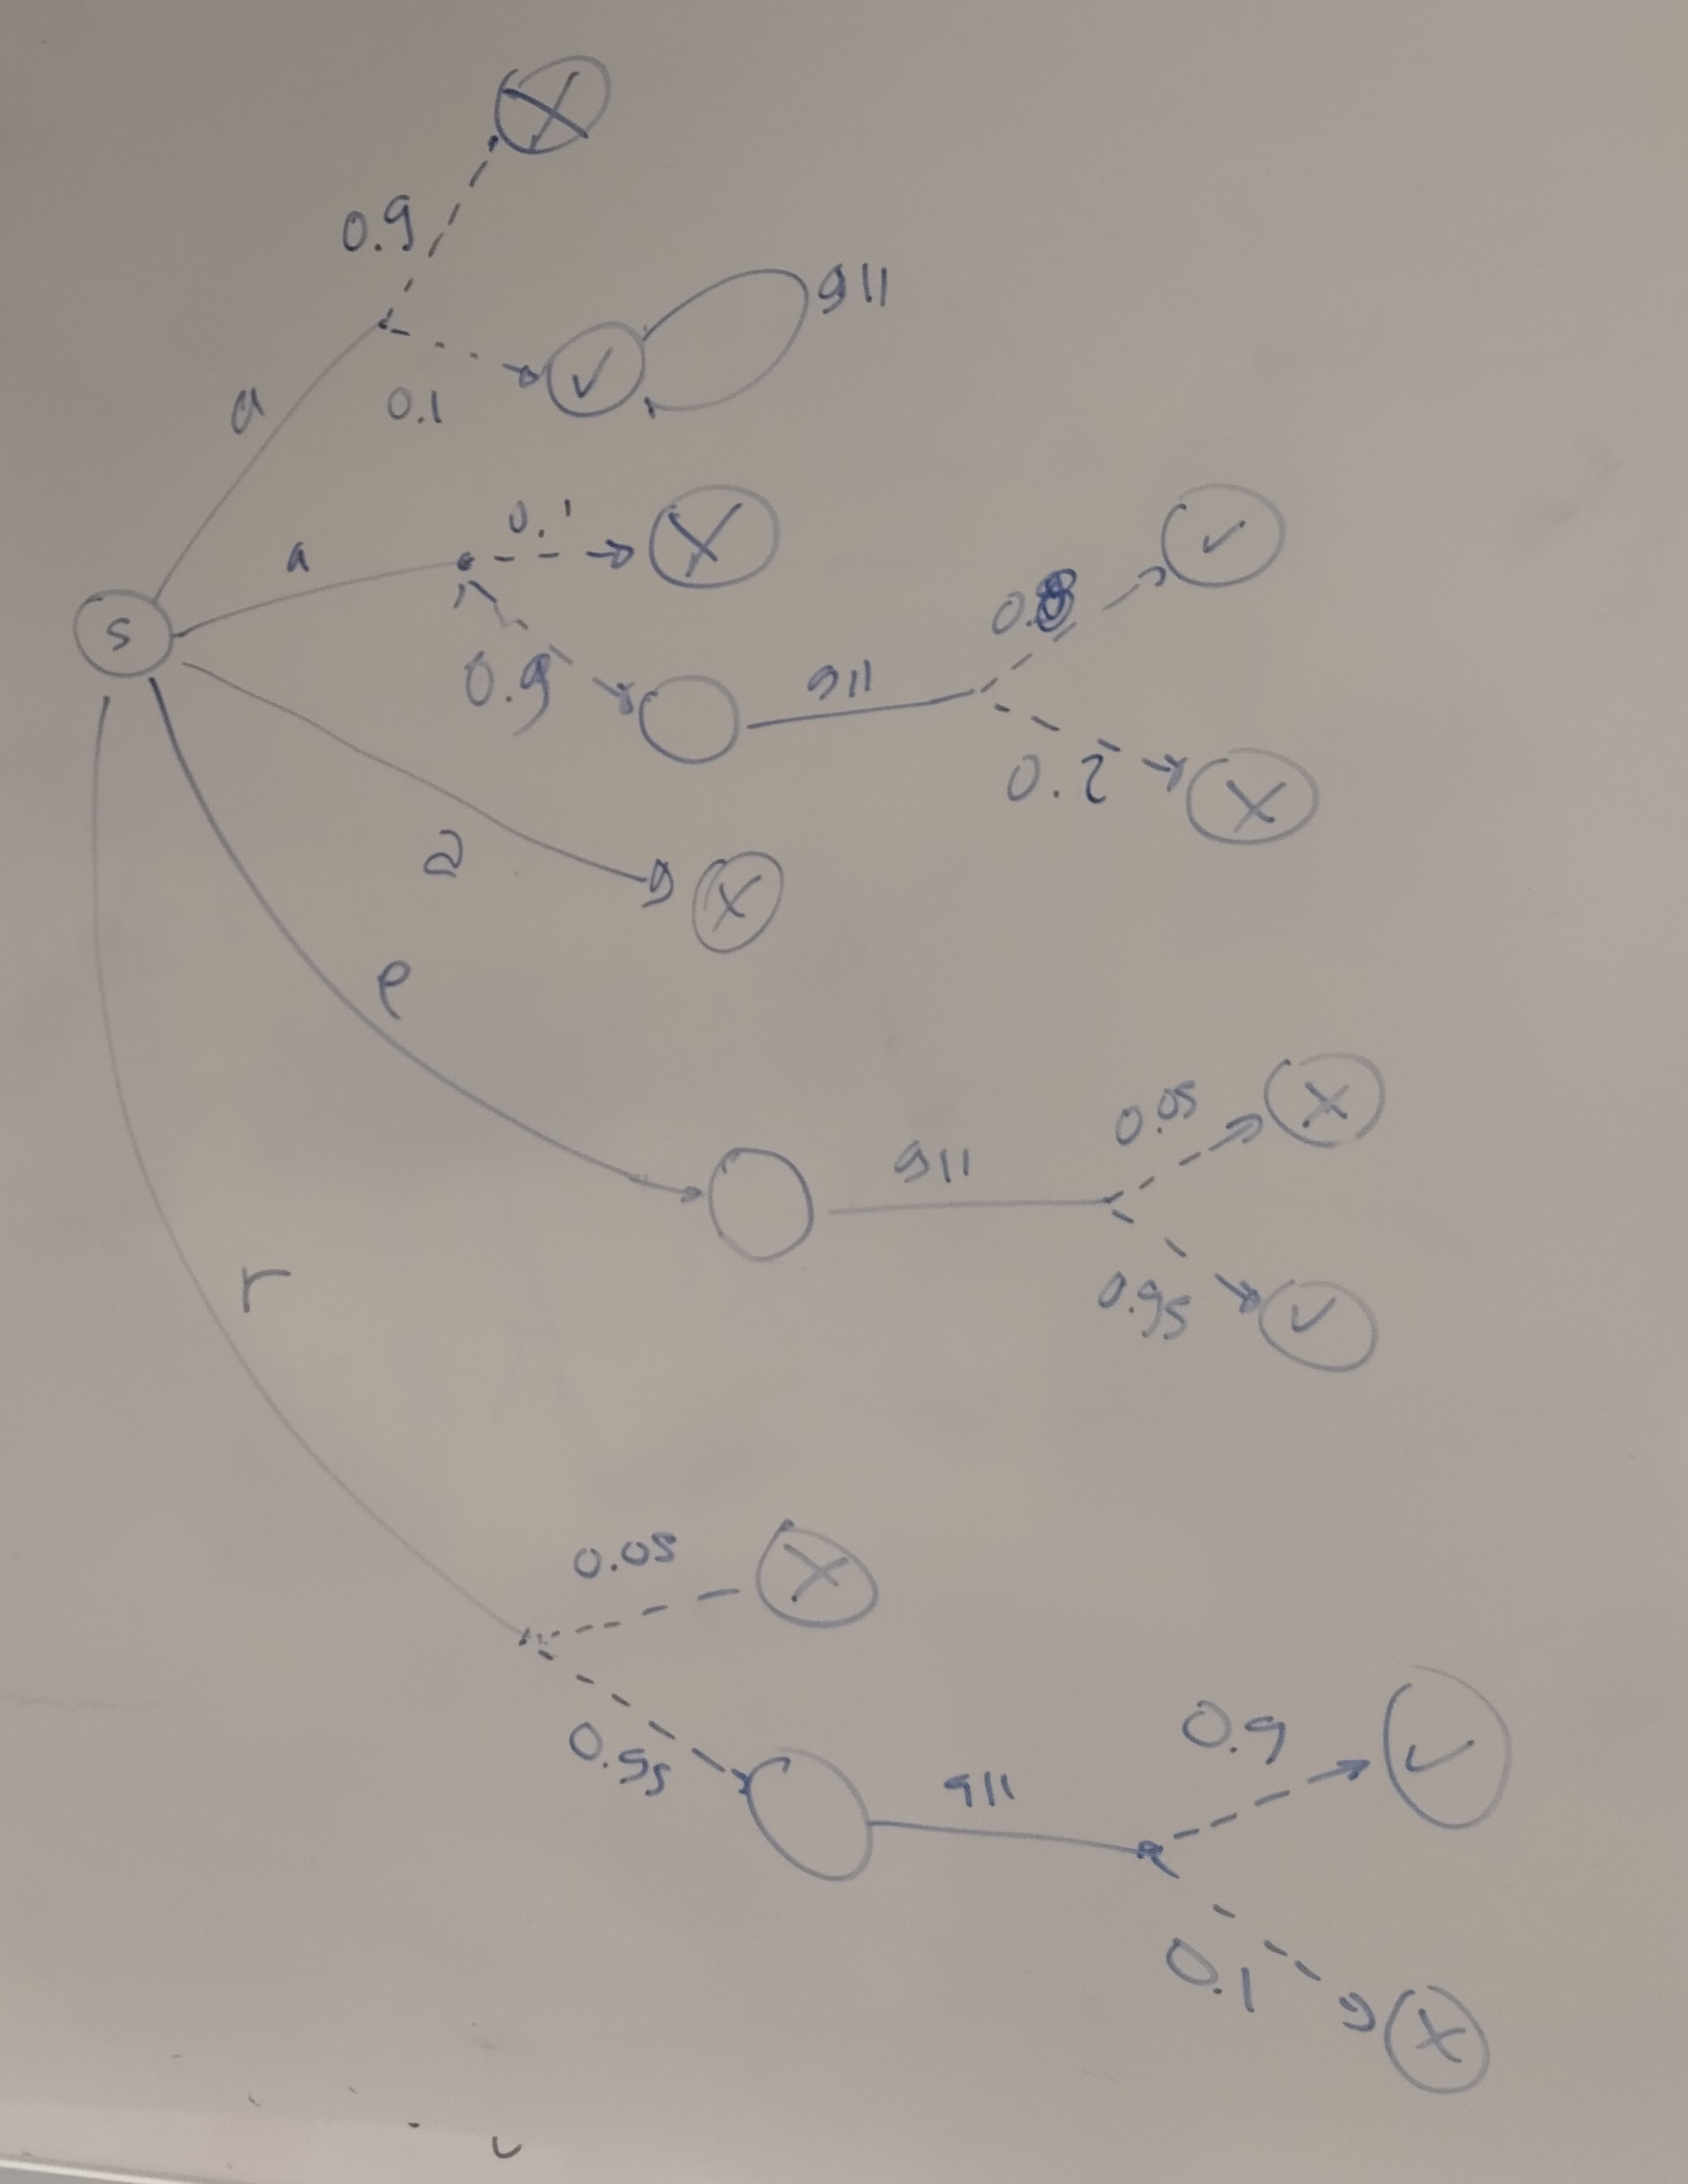
\includegraphics[scale=0.1]{PLTS.jpg}
    \end{center}
\end{figure}

% We need to capture the notion of executability with probability at least $q$, for some $q\in[0,1]$. 

% \begin{definition}\label{def:strategy-comp-exec}
%     Let $\model=\tup{\S,\Act,\ra,\V}$ be a PLTS, a \emph{strategy} is a function $\strat: \S\times(\Act\times\S)^* \ra \Dist(\S\times\Act\times\Dist(\S))$. Let $\plan\in\Act^*$, we say that $\strat$ is \emph{$\plans$-compatible} if and only if, for all $\rho\in \S\times(\Act\times\S)^*$, the following conditions hold:
%     \begin{enumerate}
%         \item $\strat(\rho)(s,a,\mu)>0$ implies $\last(\rho)=s$ and $s\reach{a}\mu$ in $\model$, and 
%         \item $\bar{\rho}\in\pref(\plans)$ implies $\bar{\rho}a\in\pref(\plans)$.
%     \end{enumerate}
%     For $\plan\in\Act^*$, we say that $\strat$ is \emph{$\plan$-compatible} if it is $\{\plan\}$-compatible. 

%     Let $q\in[0,1]$, we say that $\plans$ is \emph{$q$-executable} at $s\in\S$, if and only if, 
%     \[
%         \infim_{\{\strat \mid \strat \text{ is } \plans\text{-comp.}\}} \Prob^\strat_{s}(\plans)\geq q.
%     \]
%     Finally, $\plans$ is \emph{$q$-executable} at $B\subseteq\S$, if and only if, it is $q$-executable at every $s\in B$. 
%     A plan $\plan$ is \emph{$q$-executable} at $s$ (respectively, at $B$) if $\{\plan\}$ is $q$-executable at $s$ (respectively, at $B$). 
% \end{definition}

% \bigpedro{todo lo de arriba en esta subsecci\'on deber\'ia irse, la mayor\'ia de las cosas est\'an definidas en los preliminaries, queda la idea de $\plans$-compatible que viene debajo}



Given a set of plans $\plans\subseteq\Act^*$, we want to consider
strategies that follow as faithfully as possible the plans of
$\plans$.  Therefore, we say that a strategy $\strat$ is
\emph{$\plans$-compatible} if for all $\rho\in\execf$ such that
$\bar{\rho}\in\pref(\plans)$,
%
\begin{enumerate}
\item%
  $\strat(\rho)(a,\mu)>0$ implies $\bar{\rho}a\in\pref(\plans)$, and
\item%
  $\strat(\rho)(\complete)>0$ implies that either
  $\bar{\rho}\in\plans$ or
  $\bar{\rho}\{a\mid{\last(\rho)\reach{a}\mu}\}\cap\pref(\plans) = \emptyset$. 
\end{enumerate}
%
The first item states that $\strat$ can chose an $a$-labelled
transition after the partial plan $\bar{\rho}$ if the continuation of
$\bar{\rho}a$ is also a partial plan.
%
The second item states that $\strat$ is allowed to terminate after the
partial plan $\bar{\rho}$ if either $\bar{\rho}$ is itself a valid
plan, or $\bar{\rho}$ cannot be continued by the PLTS within some
valid plan.
%
Let $\Comp(\plans)$ denote the set of all $\plans$-compatible
strategies.
%
%% Given a plan $\plan\in\Act^*$, we say that a strategy $\strat$ is
%% $\plan$-compatible iff it is $\{\plan\}$-compatible.


Let $\plans$ be a set of plans that are believed to perform
equivalently in order to reach some goal state in $G\subseteq\S$.  We
define the set of \emph{successful complete (finite) execution} that
reach $G$ following some plan in $\plans$ by
$\Succ(\plans,G)=\{{\rho\complete\in\cexecf}\mid{\bar{\rho}\in\plans
  \text{ and } \last(\rho)\in G}\}$.
%
We are interested in that any $\plans$-compatible strategy $\strat$
starting from a given state $s\in\S$ reaches a state in $G$ with a
minimum desired probability, say $q$.  That is, we would like that
%
\begin{equation}\label{eq:plans:goal:q}
  \inf_{\strat \in\Comp(\plans)}\Prob^\strat_s(\Succ(\plans,G)) \geq q.
\end{equation}
%
More generally, we would like that this holds from any particularly
assumed state in a set $A\subseteq\S$ (say, a precondition).  So, we
write $A \reach{\plans}_q G$ if and only if for all state $s\in A$,
the condition in \cref{eq:plans:goal:q} holds.
%
Thus $A \reach{\plans}_q G$ means that any state in $A$ can reach the
goal $G$ with at least probability $q$ following some plan in $\plans$
\textcolor{red}{in an adaptively manner}.
\pedro{ejemplo de esto tambi\'en}


\bigpedro{creo que es importante pensar ahora la estructura del paper}




\bigpedro{desde el cartel hasta aqu\'i es nuevo}



Notice that, whenever $q=1$, we are in the case of SE from~\Cref{def:plans}. \raul{Chequear esto} The extended language with probabilities is given below.


\begin{definition}
    \label{def:syntax-extended}
    The set of formulas (a.k.a. the language) of $\Khlogic$ is defined by the following BNF:
    \[
        \varphi, \psi ::= p \mid \neg \varphi \mid \varphi \vee \psi \mid \kh^q(\psi,\varphi),
    \]
    where $p\in\Prop$ and $q\in[0,1]$. Other Boolean operators are defined as usual. Formulas of the form $\kh(\psi,\varphi)$ are read as \emph{``the agent knows how to achieve $\varphi$ given $\psi$ with probability at least $q$''}.
\end{definition}




Now we proceed by introducing the semantics of the new modality.

\begin{definition}
    \label{def:semantic-extended}
    Let $\model = \tup{\S,\Act,\ra,\V}$ be a PLTS and let $s\in\S$, the satisfiability relation $\models$ for $\PKh$ is inductively defined as:
    \[
        \begin{array}{l@{\ \ \ }c@{\ \ \  }l}
        % \model, s \models p & \iffdef & p \in \V(s) \\
        % \model, s\models \neg\varphi & \iffdef & \model, s \not\models \varphi \\
        % \model, s \models \psi\vee\varphi & \iffdef & \model, s \models \psi \mbox{ or }\model, w \models \varphi \\
        \model, s \models \kh^q(\psi,\varphi) & \iffdef & \text{there is } \plan \in \Act^* \;\text{such that:} \\
        & & \ \ \text{\rm (1)} \ \plan \text{ is $q$-executable at }  \truthset{\model}{\psi}\; \text{and} \\
        & & \ \ \text{\em (2)} \ \truthset{\model}{\psi} \reach{\plan}_q \truthset{\model}{\varphi}, 
        \end{array}
        \] \raul{1 and 2 will be merged into one condition.}
        where: $\truthset{\model}{\chi} := \csetsc{s\in\S}{\model,w\models\chi}$. Define: $\model\models\varphi$ iff  $\truthset{\model}{\varphi}=\S$, and $\models\varphi$ iff $\model\models\varphi$, for all PLTS $\model$.
\end{definition}

\begin{theorem}\label{th:mc-khp-undecidable}
The model-checking problem for $\PKh$ is undecidable.
\end{theorem}

\begin{proof}
    Suppose we want to check whether $\model,s\models\kh^q(\psi,\varphi)$.  W.l.o.g., consider $\model$ is complete and deterministic. 
    From the semantics, we need to check if there is $\plan\in\Act^*$ satisfying conditions (1) and (2). Consider condition (1), i.e., we need to check whether $\plan$ is $q$-executable at all $s\in\truthset{\model}{\psi}$. Fix such an $s$. Since $\model$ is deterministic and complete, it all boils down to check whether there is $\plan\in\Act^*$ such that $\Prob^\strat_s(\plan)\geq q$ (notice that $\strat$ is unique by determinism of $\model$). 
    The latter solves the problem of checking whether the language recognized by a probabilistic (deterministic) automata is empty, which is undecidable~\cite{MadaniHC99}. 
\end{proof}


\subsection{A First Approach: Non-Adaptive Plans}

The results in the above show a huge jump in the computational behaviour of knowing-how: while model-checking in the standard case is \PSPACE-complete, considering probabilities leads to undecidability of the same problem. Here, we will deal with the version of knowing-how, in which an agent only considers plans that belong to its uncertainty/awareness class. We will introduce two logics considering probabilities, one generalizing the logic from~\cite{AFSVQ21,AFSVQ23} (each plan in a class must be an appropriate plan) and another one in which it will suffice to have certain appropriate plans in a class. For the former, the model-checking problem again becomes undecidable (contrary to the \PTIME problem of the logic without probabilities, see e.g.~\cite{AFSVQ21,AFSVQ23,DF23}), while for the second, the problem is decidable. In what follows, apart from the technical results, we will motivate the use of the decidable logic in some examples.

Here we introduce some definitions, extending those in e.g.~\cite{AFSVQ21,AFSVQ23}.


\begin{definition}\label{def:plts}
    Let $\Prop$ be a countable set of propositional symbols and let $\AGT$ be a finite set of agents.  
    A \emph{Probabilistic Labeled Transition System with uncertainty (PLTSU)}  is a tuple
    $\model=\tup{\S,\Act,\ra,\sim,\V}$ s.t. $\tup{\S,\Act,\ra,\V}$ is a PLTS, and 
    \begin{itemize}
        % \item $\S$ is a countably non-empty set of states,
        % \item $\Act$ is a countable set of action symbols,
        % \item $\Dist(\S)$ is the set of probability distributions over $\S$,
        % \item ${\ra} \subseteq \S \times \Act \times \Dist(\S)$ is a transition relation,
        \item ${\sim}\subseteq \DS{}\times \DS{}$ (where $\DS{}\subseteq\Act^*$) is an equivalence relation over $\DS{}$. 
        % \item $\V: \S \ra 2^\Prop$ is a valuation function.
    \end{itemize}
    %Elements of $\Act^*$ are called \emph{plans}, and 
    Each $\sim$ is called the indistinguishability relation between plan. 
    % We write $\plan\sim_i\plan'$ whenever $(\plan,i,\plan')\in{\sim}$, and we define $\DS{i}:=\set{\plan \mid \text{ there is } \plan' \text{ s.t. } \plan\sim_i\plan'}$. 
    By $[\plan]_{\sim}:=\set{\plan' \in \DS{} \mid \plan \sim_i \plan'}$ we denote $\plan$'s equivalence relation with respect to $\DS{}$, then we define the \emph{indistinguishability set of $\model$} as $\Unc := \set{[\plan]_{\sim} \mid \plan\in\DS{}}$. 
    %The set $\Unc:=\set{\Unc(i) \mid i\in\AGT}$ is called the \emph{uncertainty set} of $\model$. 
    For simplicity sake, we sometimes denote $\model=\tup{\S,\Act,\ra,\Unc,\V}$ to refer to a PLTS, i.e., we will use its uncertainty set instead of the indistinguishability relation.
\end{definition}

Notice that, as it is defined in~\cite{AFSVQ21,AFSVQ23}, $\Unc$ represents the perception the agent has about the reality. In turn, the relation $\sim$ is not an equivalence relation over $\Act^*$ but over $\DS{}$, as the latter contains only the plans she considers available or suitable for her purposes, while those in $\Act^*\setminus\DS{}$ are not considered by the agent, even if they are suitable plans. 

% \begin{definition} \label{def:executability} \raul{TBC}
%     Let  $\model=\tup{\S,\Act,\Dist(\S),\ra,\Unc,\V}$ be a PLTSU, let $\plan\in\Act^*$ be a plan, and let $q\in[0,1]$ a probability, we need to define two notions:
%     \begin{enumerate}
%         \item We say $\plan$ is \emph{$q$-executable} at $s\in\S$ iff ...  Extend it for set of plans and set of states.
%         \item For $s,t\in\S$, we write $s \reach{\plan}_q t$ iff ... Extend it for set of plans and set of states.
%     \end{enumerate}
% \end{definition}

In general, we will assume that PLTS are complete, as for those we can always complete the execution of a plan to a \emph{sink state}.

% \begin{definition}
%     \label{def:syntax}
%     The set of formulas (a.k.a. the language) of $\PKhunc$ is defined by the following BNF:
%     \[
%         \varphi, \psi ::= p \mid \neg \varphi \mid \varphi \vee \psi \mid \kh_i^q(\psi,\varphi),
%     \]
%     where $p\in\Prop$, $i\in\AGT$ and $q\in[0,1]$. Other Boolean operators are defined as usual. Formulas of the form $\kh_i^q(\psi,\varphi)$ are read as \emph{``agent $i$ knows how to achieve $\varphi$ given $\psi$, with probability $q$''}
% \end{definition}

\begin{definition} \label{def:semantics-non-adap}
    Let $\model = \tup{\S,\Act,\ra,\Unc,\V}$ be a PLTSU and let $s\in\S$, the satisfiability relation $\models$ for $\PKhunc$ is inductively defined as:
    \[
    \begin{array}{l@{\ \ \ }c@{\ \ \  }l}
    % \model, s \models p & \iffdef & p \in \V(s) \\
    % \model, s\models \neg\varphi & \iffdef & \model, s \not\models \varphi \\
    % \model, s \models \psi\vee\varphi & \iffdef & \model, s \models \psi \mbox{ or }\model, w \models \varphi \\
    \model, s \models \kh^q(\psi,\varphi) & \iffdef & \text{there is } \plans \in \Unc \;\text{such that for all } \plan\in\plans{:} \\
    & & \ \ \text{\rm (1)} \ \plan \text{ is $q$-executable at }  \truthset{\model}{\psi}\; \text{and} \\
    & & \ \ \text{\em (2)} \ \truthset{\model}{\psi} \reach{\plan}_q \truthset{\model}{\varphi}, 
    \end{array}
    \]     \raul{1 and 2 to be merge into one.}
    \noindent where: $\truthset{\model}{\chi} := \csetsc{s\in\S}{\model,w\models\chi}$. Define: $\model\models\varphi$ iff  $\truthset{\model}{\varphi}=\S$, and $\models\varphi$ iff $\model\models\varphi$, for all PLTS $\model$.
\end{definition}

This definition bears a resemblance to the one in Section~\ref{sec:khlinearplans}, except that we ask the conditions hold for \emph{every plan} belonging to a set of indistinguishable plans $\plans$. We call this version of the logic \emph{non-adaptive} for such a reason, as the agent cannot use the ``good plans'' whenever she considers them ``equally good'' as others.  We will discuss later an alternative to this notion.

For this logic, we obtain a result similar to the one in the previous section.

\begin{theorem}\label{th:mc-khp-nadapt-undecidable}
    The model-checking problem for $\PKhunc$ under the semantics from Definition~\ref{def:semantics-non-adap} is undecidable.
\end{theorem}


\subsection{A Second Approach: Adaptive Plans}

Now we introduce a version of the logic $\PKhunc$ in which suitable plans for achieving a goal are \emph{adaptive}, in the sense that the full set $\plans$ must be $q$-executable, and not each plan $\plan\in\plans$ separately. Thus, the agent can use those plans that are good for her purposes, even in presence of non-appropriate plans that she considers indistinguishable from the good ones. \raul{Esto hay que venderlo un poco mejor.}

\begin{definition} \label{def:semantics-adap}
    Let $\model = \tup{\S,\Act,\ra,\Unc,\V}$ be a PLTSU and let $s\in\S$, the satisfiability relation $\models$ for $\PKhunc$ is inductively defined as:
    \[
    \begin{array}{l@{\ \ \ }c@{\ \ \  }l}
    % \model, s \models p & \iffdef & p \in \V(s) \\
    % \model, s\models \neg\varphi & \iffdef & \model, s \not\models \varphi \\
    % \model, s \models \psi\vee\varphi & \iffdef & \model, s \models \psi \mbox{ or }\model, w \models \varphi \\
    \model, s \models \kh^q(\psi,\varphi) & \iffdef & \text{there is } \plans \in \Unc \;\text{such that:} \\
    & & \ \ \text{\rm (1)} \ \plans \text{ is $q$-executable at }  \truthset{\model}{\psi}\; \text{and} \\
    & & \ \ \text{\em (2)} \ \truthset{\model}{\psi} \reach{\plans}_q \truthset{\model}{\varphi}, 
    \end{array}
    \]     \raul{1 and 2 to be merge into one.}
    \noindent where: $\truthset{\model}{\chi} := \csetsc{s\in\S}{\model,w\models\chi}$. Define: $\model\models\varphi$ iff  $\truthset{\model}{\varphi}=\S$, and $\models\varphi$ iff $\model\models\varphi$, for all PLTS $\model$.
\end{definition}

The general idea in condition 1 of the clause for $\kh$ establishes that all the plans in $\plans$ have a probablity of at least $q$ of succeeding. Since all plans in $\plans$ are indistinguishability, this needs to be guaranteed no matter which plan is chosen. However, there are at least two alternatives in this definition: one considering \emph{adaptability}, meaning that there is at least one possible execution of each plan in $\plans$ for which probability $q$ is guaranteed, and considering \emph{non-adaptability} whenever we need this guarantee on each possible execution of every plan in $\plans$. Condition 2 establishes that successfull states are reached with probability of at least $q$.

\begin{remark}
    Notice that an equivalence class $\plans$ can be defined in terms of a Deterministic Finite State Automata (DFA) $\mathcal{A}_{\plans}$. This way, the operation of checking $q$-executability can be perfomed over the product $\model\times\mathcal{A}_{\plans}$. In short, $\plans$ is $q$-executable at $s$ iff for each $\plan\in\plans$, there exists one MDP in  $\model\times\mathcal{A}_{\plans}$ in which the probability of executing $\plan$ is at least $q$. This will be used while designing a model-checking algorithm (connected with algorithms from~\cite{AFSVQ21,AFSVQ23,DF23}).
\end{remark}

\begin{theorem}\label{th:mc-khp-adapt-decidable}
    The model-checking problem for $\PKhunc$ under the semantics from Definition~\ref{def:semantics-adap} is decidable. Moreover, if each $\plans\in\Unc$ is given as input as a deterministic FSA, the problem is in $\PTIME$.
\end{theorem}
